\section{Related Work}

Researchers have long realized that incomprehensible type errors result as a consequence of standard approaches to the type inference process. Haack and Wells~\cite{haack2004type} noted that ``\textit{Identifying only one node or subtree of the program as the error location makes it difficult for programmers to understand type errors. To choose the correct place to fix a type error, the programmer must find all the other program points that participate in the error.}'' Researchers have proposed solutions to improve the type inference process. Type error slicing~\cite{haack2004type} is a technique that finds locations that are complete and minimal for the type error. Internally labeled constraints and MUS manipulation are used to generate these slices. The language supported in Haack's work was a subset of standard ML. The original Chameleon~\cite{stuckey2003interactive} used a similar technique but extended it to support advanced type-level features (type classes and functionally dependent types). The project also introduced the ability to query type information through a command line-style interface (Fig.~\ref{fig:original-chameleon}). Although Chameleon was firmly grounded in results from type theory, its designs were never evaluated with user studies.


% \begin{figure}[h]
%     \centering
%     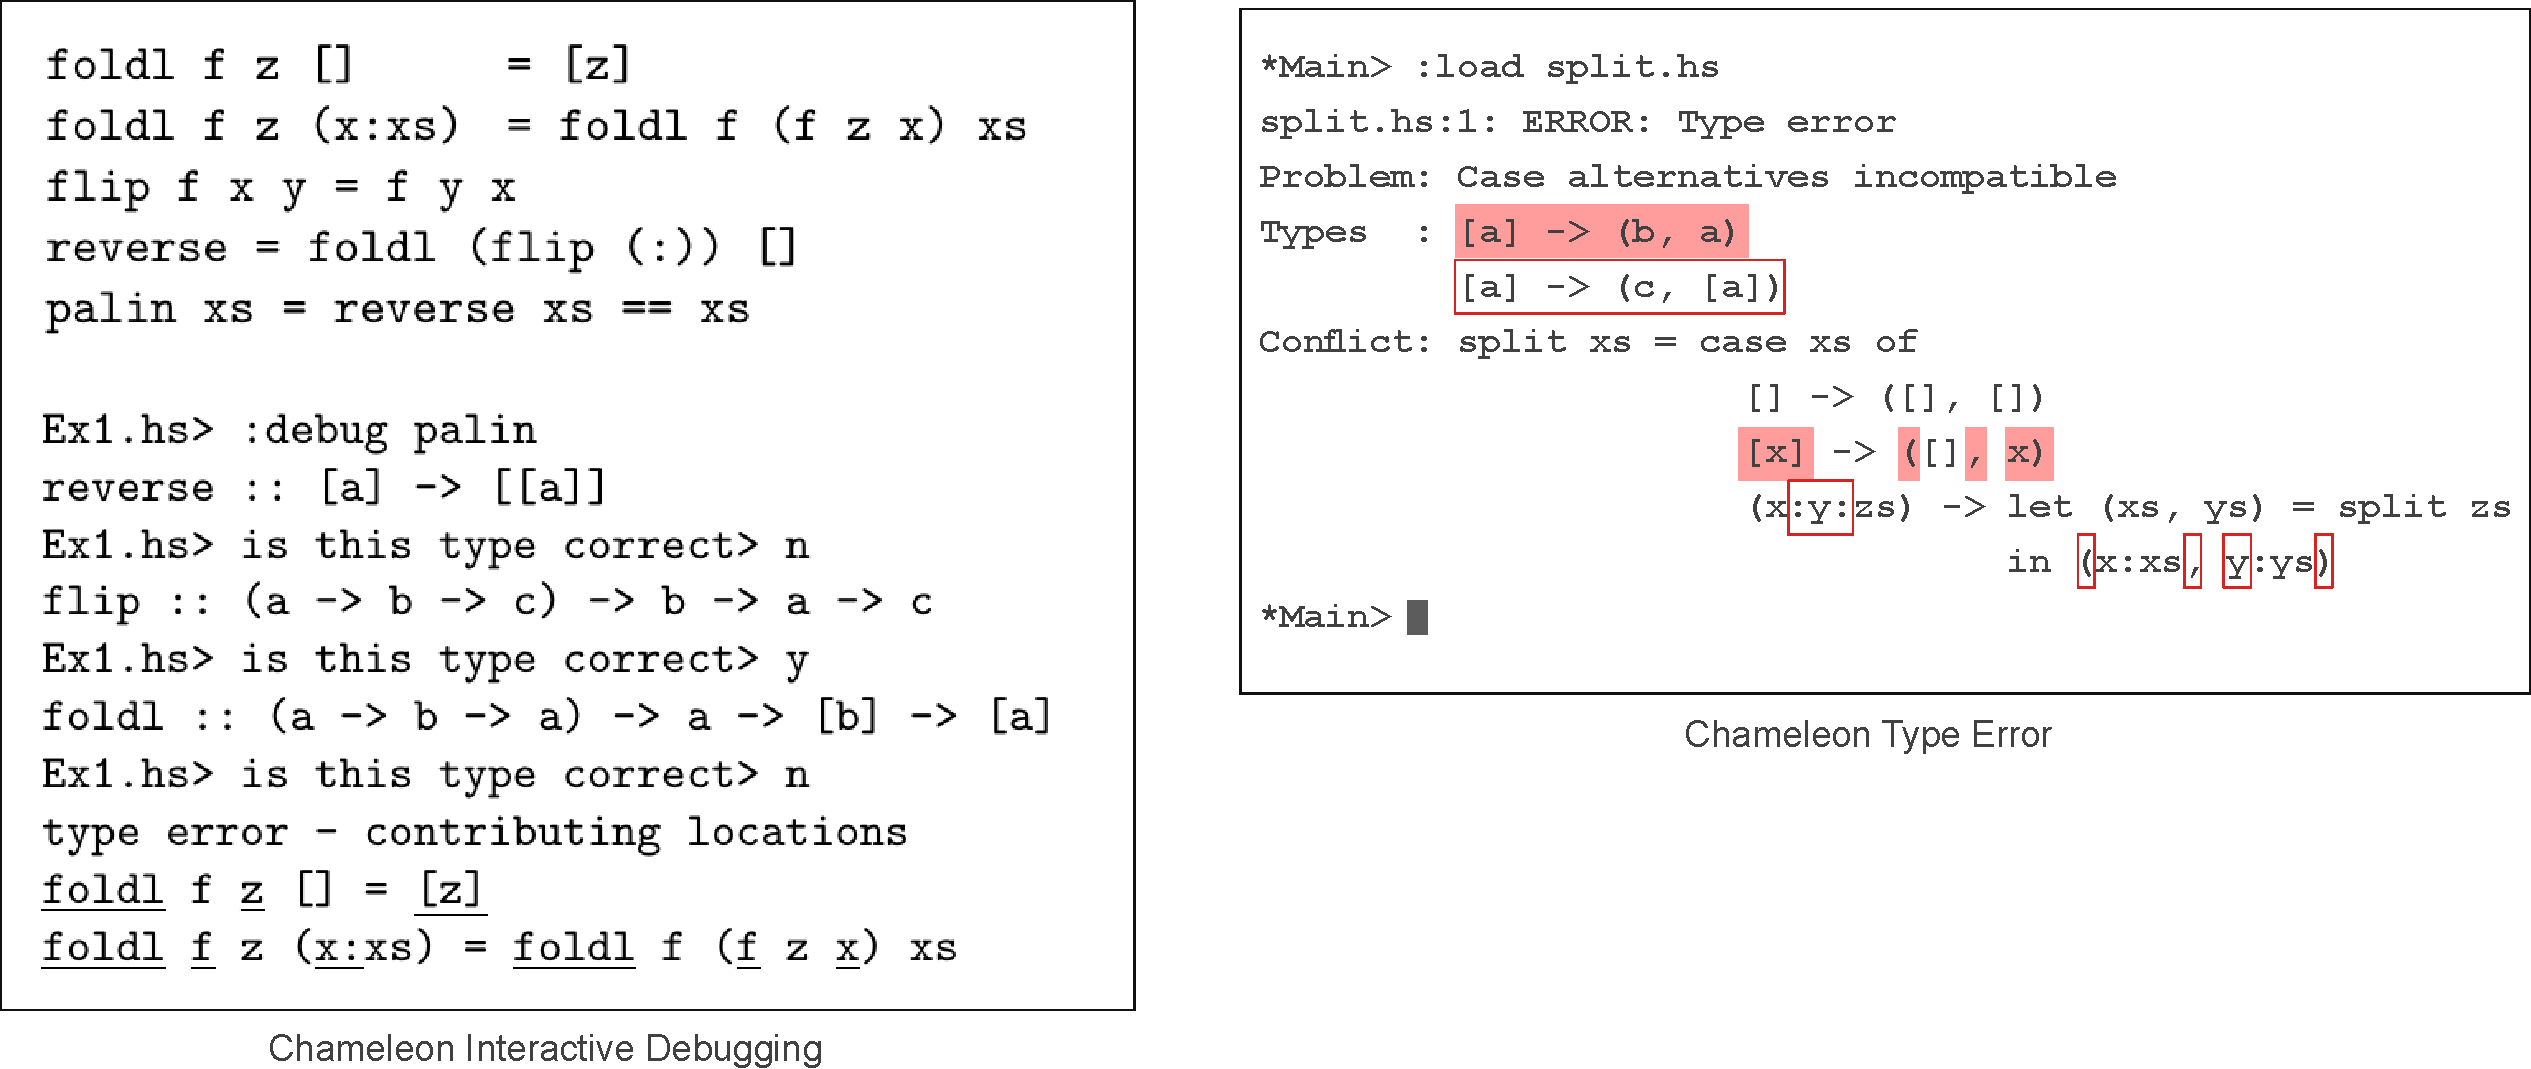
\includegraphics[width=\linewidth]{images/original-chameleon.pdf}
%     \caption{
% Originally, Chameleon was a command-line tool that can list all the potential causes of a type error and display the two branches in two forms of highlight (right), achieved with ASCII colors. In addition, it allows a few commands (debug and explain) in the debugging shell to help debug type errors (left).}
%     \label{fig:original-chameleon}
% \end{figure}


% The ChameleonIDE error reporting The error message of ChameleonIDE closely
% follows the argumentation structure outlined by Titus. Basic mode represent a
% simple structure argument, where the claim "The expression e can have two
% conflicting types" and the possible type 1 and two serves as grounds. When
% inspecting each possible types, the type judgements are treated as claim, and it
% is supported by the grounds: "Inferred from the orange/blue highlights on the
% left side". On the other hand, the similar type error message in GHC "Couldn't
% match expect type T1 with actual type T2" is "a ground masquerading as a clam",
% Barik commented. The balanced mode and advanced mode serve as a way to elaborate
% arguments from simple arguments into extended arguments.

Another related topic is type-explanation~\cite{yang1999explaining, jun2002explaining}. Yang~\cite{jun2002explaining} showed an alternative type inference system capable of producing a human-like text explanation for why expressions are assigned certain types. A good explanation is drawn from surveying how human experts explain types. The resulting algorithm $\mathcal{H}$, generates a succinct explanation of the type inference steps to avoid using internal constructs (such as type variables). The explanation system has the advantage of acting like a human expert. However, when presented as text-based output, explanation systems have the potential to become verbose when types are complex or variable names are long. In \chameleon{}, we attempt to address this problem by showing one step of explanation at a time and referring to variables instead of spelling out the full name.

% Another method to improve type error message is search based type
% checking~\cite{lerner2007searchingtypeerror}. This method incrementally modifies
% an ever smaller part of the abstract syntax tree and replacing it with a
% wildcard expression and querying the type checker to verify if the program still
% type-checks. Lerner's study showed how two implementations could provide
% high-quality error messages and to suggest accurate fixes. While this system is
% great for suggesting solutions, is it limited in its ability to explain the type
% errors due to the fact that the system is unaware of any inner workings of the
% type systems. 


% Some studies \cite{seidel2017learningtoblame} proposed a heuristic approach to
% improve type error messages. These studies use part of type information in the
% program to query external databases. Based on the external databases'
% capability, some projects can interactively fix the type error on the fly with
% reasonable accuracy. \pjs{Add jusdgment/comparison sentence!}



Debugging using a GUI Interactive Development Environment has been the standard practice for a very long time. Compared to a command line-based interface, a graphic user interface provides programming tools with the ability to show information hierarchy, provide immediate feedback to changes, and display complex visualizations. RxFiddle~\cite{banken2018debugging} is a tool to visualize data flow and value changes in a functional reactive program. Whyline~\cite{ko2009finding} is a Java debugging system that allows a user to ask questions like "why does variable X have value Y". It also allows users to interactively ask follow-up questions to gain further knowledge of the nature of an error. Both  systems target programming runtime systems instead of types systems and static analysis. In fact, support for type systems has been lacking in both academic and industry software engineering tool design. The most common approach for supporting type systems we see in current programming editors and IDEs is to display type annotations when hovering on an expression and show a squiggly line to indicate the type error location. In \chameleon{}, colours and geometric shapes are used to create visual clarity of different components of a type error; interactivity is used to show conditional information and to change the granularity of details.


